\documentclass{article}
\usepackage[utf8]{inputenc}
\usepackage[T1]{fontenc}
\usepackage{graphicx}
\usepackage{amsmath}
\usepackage{wrapfig}
\usepackage[top=1in, bottom=1.25in, left=1.1in, right=1.1in]{geometry}

\title{Reporte - Actividad 8: Oscilador de Van der Pol}
\author{García Monge Itzel Alexia}
\date{12 de Marzo, 2018}

\begin{document}
\maketitle
\section{Introducción}
La Teoría de Sistemas Dinámicos apareció por primera vez en el siglo \textit{XVII} al introducir Newton el concepto de ecuaciones diferenciales ordinarias, pero no es sino hasta el siglo \textit{XIX} que Henri Poincaré se vuelve el padre de la teoría moderna de los sistemas dinámicos, seguido por I. Bendixson con el estudio de las propiedades topológicas de las ecuaciones diferenciales odrinarias autónomas en el plano.

 B. Van del Pol fue un físico e ingeniero eléctrico holandés que realizó un gran aporte a la \textit{Teoría de Sistemas Dinámicos} al encontrar oscilaciones estables, mejor conocida como ciclos límites estables en circuitos eléctricos con tubos de vacío.

El \textit{osciador de Van del Pol} modela un circuito eléctrico usado en varias áreas como la biología para las potencialidades de acción de neuronas; la medicina para construir una serie de modelos de circuitos eléctricos del corazón humano para estudiar su rango de estabilidad dinámica; en la matemáticas y física el nombre de van del Pol está asociado a una ecuación diferencial ordinaria de segundo orden de la forma:

\[\ddot{x} - \varepsilon (1 - x^2) \dot{x} + x = 0 , \varepsilon \text{   positivo} \]

\section{Modelo de Van der Pol}
\subsubsection{Historia}
El oscilador de Van del Pol fue propuesto originalmente por el ingeniero eléctrico y físico Balthasar van del Pol. Van del Pol encontró oscilaciones, llamándolas oscilaciones de relajación, las cuales son conocidas como un tipo de ciclo límite en circuitos eléctricos utilizando tubos de vacío. Cuando estos circuitos se acercan al ciclo límite, la señal envía una corriente con ella. Van del Pol y Van der Mark, el cual era un colega, reportaron que a cierta frecuencias se escuchaba un ruido irregular. Este ruido pasó a ser el resultado del caos determinístico.

Su ecuación tiene ha sido usado usada en las ciencias tanto físicas como biológicas, además de ser usada en sismología y en estudios de fonética.


\subsubsection{Forma Dos-Dimensional}
El Teorema de Liénard puede ser usado para probar que el sistema tiene un ciclo límite. Aplicando la transformación de Liénard $y = x - \frac{x^3}{3} - \frac{\dot{x}}{\mu}$  donde el punto representa la primera derivada, el oscilador de Van del Pol puede escribirse en su forma dos dimensional:

\[dot{x} = \mu (x - \frac{x^3}{3}) - y \]

\[\dot{y} = \frac{x}{\mu} \]

Otra forma base comúnmente utilizada en la transformación :
\[\dot{x} = y \]

\[\dot{y} = \mu (1 - x^2 )y - x \]


\subsubsection{Resultados para un Oscilador sin Forzamiento}
El oscilador de Van del Pol sin forzamiento tiene dos características interesantes, las cuales están ligadas con el amortiguamiento. 

\begin{itemize}
\item Cuando $\mu$=0 no hay amortiguamiento, volviéndose un simple oscilador armónico al no haber oscilaciones forzadas donde siempre hay conservación de la energía. Su ecuación se vuelve de la forma:
\[ \frac{d^2x}{dt^2} + x = 0 \]

\item Cuando $\mu$ $\>$ 0 el sistema entrará a un ciclo límite. Cerca del origen el sistema es inestable, mientras que fuera del origen el sistema tiene amortiguamiento.

\end{itemize}


\subsubsection{Hamiltoniano para el oscilador de Van del Pol}
Si deseáramos escribir la ecuación de Van der Pol con un Hamiltoniano independiente del tiempo, aumentando a un sistema dinámico autónomo de cuatro dimensiones, obtendríamos la ecuación diferencial auxiliar no lineal:

\[ \ddot{x} - \mu(1 - x^2)\dot{x} + x = 0 \]

\[ \ddot{y} + \mu(1 - x^2)\dot{y} + y = 0 \]

Un Hamiltoniano $H$ para este sistema de ecuaciones es:

\[ H(x, y, p_x, p_y) = P_x P_y + xy - \mu(1 - x^2)yp_y \]


\subsubsection{Oscilador de Van del Pol Forzado}
El oscilador de Van del Pol forzado toma la ecuación original y le agrega la función A($\omega$t), donde $A$ es la amplitud y $\omega$ es la velocidad angular, para dar la ecuación diferencial:

\[ \frac{d^2}{dt^2} - \mu(1 - x^2)\frac{dx}{dt} + Asin(\omega t) = 0 \]


\subsubsection{Forzamiento Periódico y Caos Determinístico}
La ecuación del oscilador Van del Pol con un forzamiento periódico está formulado como:

\[ \ddot{x} - \mu(1 - x^2)\dot{x} + x = Fcos\frac{2 \pi t}{T_{in}} \]

Caos puede ser encontrado en el sistema cuando la no linealidad del sistema es lo muy fuerte. Si se gráfica, se puede observar que el caos toma lugar en los rangos estrechos de $\mu$.

Se cree hoy en día que Van der Pol y Van der Mark escucharon el caos determinístico al crear un circuito eléctrico compuesto por una resistencia, capacitancia y una lámpara de $Ne$. Tiempo después, Lorenz publicó la imagen de un atractor caótico en el espacio fase.

El modelo de Van del Pol fue simulado usando computaciones de alta resolución, identificando que las regiones que se superponían en el dominio del parámetro eran similares a la lengua de Arnold. Esto motivó una investigación exitosa del ciclo límite en tejido neural.



\section{Exploración de las soluciones del modelo en el Espacio Fase}
Se trabajaron con tres celdas base para la creación de todas las gráficas en esta actividad basándose en el código realizado en actividades anteriores. 

Primeramente se creó una celda que tuviera un campo vectorial donde se escribió la ecuación de Van der Pol, pues ese es el sistema de ecuaciones que se quiere resolver. Después, se agregó una segunda celda donde se escriben los valores de los parámetros, el tiempo y las condiciones iniciales. La última celda base fue la creación de las gráficas en si.

Para comprobar si verdaderamente el ciclo límite convergía a la misma figura con cualquier condición inicial en el espacio fase, se crearon aisladamente cinco gráficas con condiciones iniciales aleatorias y se compararon con la gráfica obtenida. 

Las gráficas creadas obtuvieron la forma:
	\begin{center}
    \includegraphics[height=5cm]{Image1_1.png}
    \includegraphics[height=5cm]{Image1_2.png}
    \includegraphics[height=5cm]{Image1_3.png}
    \includegraphics[height=5cm]{Image1_4.png}
    \includegraphics[height=5cm]{Image1_5.png}
    \end{center}

Entonces podemos observar claramente como, sin importar que valor le damos inicialmente a  las condiciones iniciales, siempre termina creando la misma figura después de un cierto periodo de tiempo transcurrido, a diferencia de las gráficas que se obtenían en la actividad pasada, donde el cambiar ligeramente con una condición inicial creaba una figura completamente distinto.


\section{Resultados y discusión}
A continuación se muestran las gráficas obtenidas de las ecuaciones de Van del Pol con su código correspondiente de $Python$ mediante el uso de $Jupyter Lab$. 

Las primeras gráficas que se debían obtener eran las gráficas de fase mostrando el ciclo límite, el que como hemos visto, siempre converge a la misma figura después de un cierto periodo de tiempo.
Para comprobar que, al conservar un mismo amortiguamiento, sin importar las condiciones iniciales, el ciclo límite es el mismo, se superpusieron una sobra la otra, resaltando en rojo el mismo ciclo límite. 

Creamos el espacio vectorial con la ecuación de Van del Pol, haciendo a $ \mu = p$
	\begin{center}
    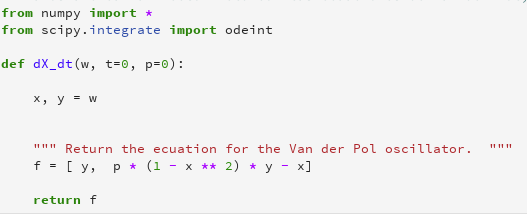
\includegraphics[height=4cm]{celda1.png}
    \end{center}

Para la segunda celda, se repite el mismo proceso, pero cambiando el nombre del archivo y modificando las condiciones iniciales.
    \begin{center}
    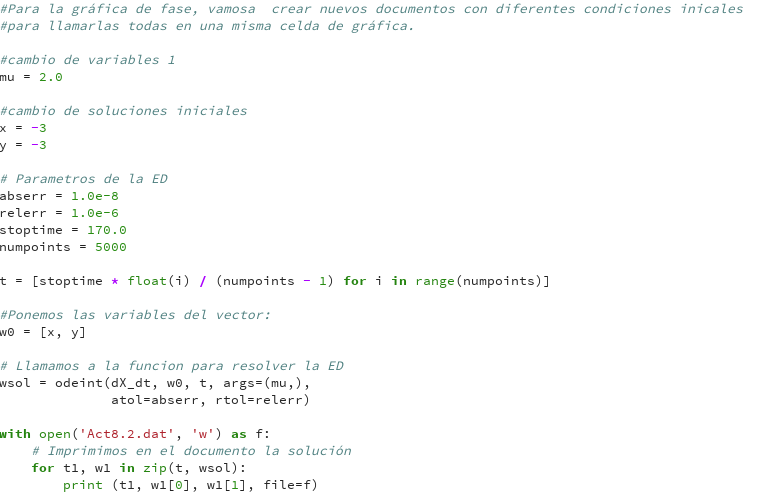
\includegraphics[height=6cm]{celda2.png}
    \end{center}
    
Al momento de graficar todas las gráficas en un mismo espacio, abrimos todos los archivos creados en la misma celda.
    \begin{center}
    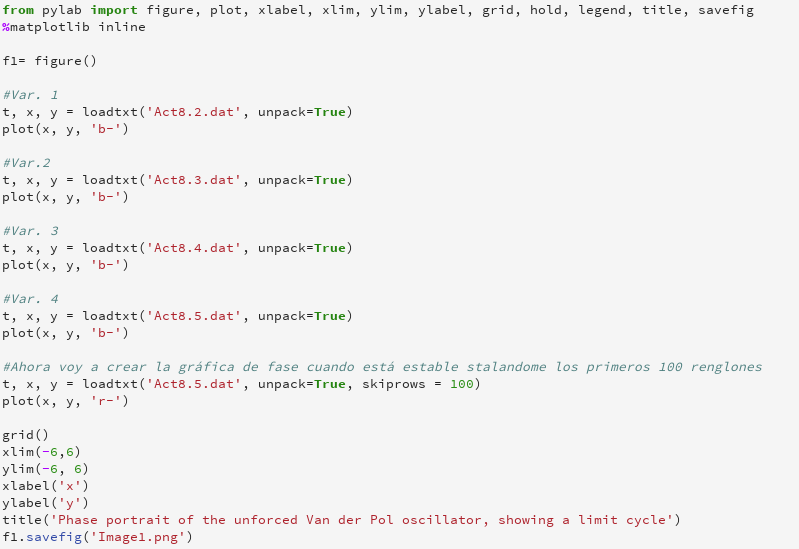
\includegraphics[height=6cm]{celda3.png}
    \end{center}
    
Finalmente, se obtuvo la gráfica
	\begin{center}
    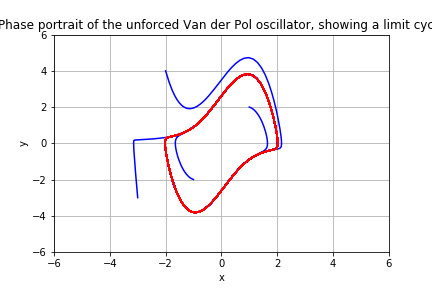
\includegraphics[height=6cm]{Image1.png}
    \end{center}

La siguiente gráfica mostró, utilizando las mismas tres celdas base de código, el ciclo límite en un plano fase. Este comenzaba como un círculo, pero conforme se modificaron los valores de $\mu$ en la segunda celda--siendo este el único cambio de valor realizado en el código--se iba extendiendo, creando un ejemplo del oscilador de relajación.

	\begin{center}
    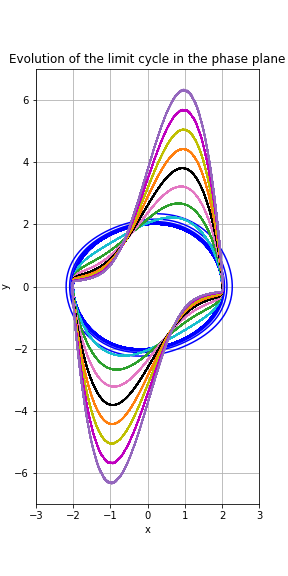
\includegraphics[height=10cm]{Image2.png}
    \end{center}
    
La tercera gráfica es un oscilador con $\mu$=5, así que nuevamente sólo se cambio el valor del amortiguamiento de la segunda celda y se graficó.

	\begin{center}
    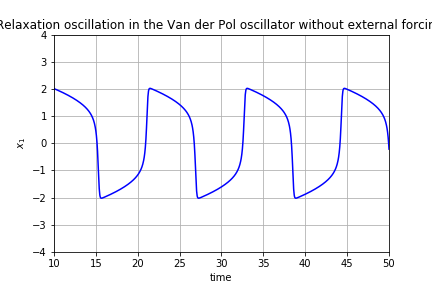
\includegraphics[height=6cm]{Image3.png}
    \end{center}

Para última gráfica se tuvo que cambiar la ecuación de Van del Pol ubicada en la primera celda de código. Se le agregaron dos parámetros nuevos que actuarían como constantes: Amlitud \textit{A} y frecuencia angular \textit{ $\omega$ }, siendo sus valores 1.2 y $\frac{2\pi}{10}$ respectivamente. La añadición de estos dos nuevos valores crea un comportamiento caótico en el oscilador de Van del Pol con forzamiento sinusoidal, siendo el amortiguamiento no lineal $\mu$=8.53. 

	\begin{center}
    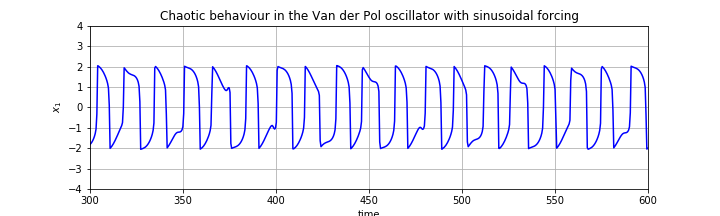
\includegraphics[height=5cm]{Image4.png}
    \end{center}

\section{Conclusión}
El oscilador de Van del Pol abre las puertas a la teoría del caos tras encontrar un valor que de un resultado de caos determinista. Esto se debe a que sus ecuaciones, al cambiar el amortiguamiento o condiciones iniciales, nos permite encontrar un comportamiento específico con el cual se encuentra información que antes no era tan fácil de apreciar, como lo es el ciclo límite. El uso de $Pytho$ y $Jupyter lab$ permitiendo una recreación donde es fácil observar que en realidad un ligero cambio lleva a algo nuevo.



\section{Bibliografía}
\begin{itemize}
\item Solución de la ecuación de Van der Pol a través de la Teoría de Sistemas Dinámicos. (Mayo 2010). Zorely A. Jesús I. Retrieved April 13, 2018.

$http://saber.ucv.ve/bitstream/123456789/12334/1/TEG \% 20Zorely \% 20A. \% 20Jes \% C3 \% BAs \% 20I..pdf$

\item Van del Pol Oscilator. (2018). Retrieved April 13, 2018.

$https://en.wikipedia.org/wiki/Van_der_Pol_oscillator$

\item Van der Pol and the history of relaxation oscillations: toward the emergence of a concept. (August 22, 2014). Jean-Marc Ginoux. Retrieved April 13, 2018.

$https://arxiv.org/pdf/1408.4890.pdf$

\item Van der Pol oscillator. (2007). Takashi Kanamaru. Retrieved April 13, 2018.

$http://www.scholarpedia.org/article/Van_der_Pol_oscillator$

\end{itemize}


\section{Apéndice}
\begin{enumerate}
\item \textbf{Este ejercicio pareciera similar al desarrollado en las actividades 6 y 7. ¿Qué aprendiste nuevo?} Traté de crear una gráfica con un campo de vectores, pero no logré hacerlo, siento que eso debía ser uno de mis logros más notorios para esta actividad. Además, aprendí a relacionar similitudes entre códigos para crear nuevos con propósitos distintos.

\item\textbf{¿Qué fue lo que más te llamó la atención del oscilador de Van der Pol?} Que no importaba cuanto cambiaras sus condiciones iniciales e incluso el amortiguamiento, su forma no era tan facilmente deformable como lo fue con las gráficas de las actividades anteriores.

\item\textbf{Has escuchado ya hablar de caos. ¿Por qué sería importante estudiar este oscilador?} Abre la puerta, como una introducción, a un tema que es muy importante en la fśicia y ciencia moderna. Es algo que se debe manejar y saber siendo un físico.

\item\textbf{¿Qué mejorarías en esta actividad?} El apoyo para recrear el campo vectorial de la imagen 1, ya que no importa cuanto le moví o a quién le pregunté, no pude recrearlo.

\item\textbf{¿Algún comentario adicional antes de dejar de trabajar en Jupyter con Python?} Fue una muy cómoda forma de trabajar, si pudiéramos retomarlo con más tiempo sería muy bueno.

\item\textbf{Cerramos la parte de trabajo con Python ¿Que te ha parecido?} Me gustó mucho la forma de escribir código por partes en celdas y el hecho de que puedas partir tu código en diferentes ventanas para no tener todo amontonado en un mismo lugar. Me gustaría seguir trabajando con un editor tan ordenado.

\end{enumerate}
\end{document}
